\documentclass[border=6pt,tikz]{standalone}
\usepackage{tikz}
\usepackage{amsmath,amssymb}
\usetikzlibrary{arrows.meta,positioning,fit,backgrounds,calc,shapes.geometric,decorations.pathreplacing,patterns}
\definecolor{ink}{HTML}{1B2430}
\definecolor{muted}{HTML}{6B7785}
\definecolor{accent}{HTML}{2F6FB5}
\definecolor{accent2}{HTML}{C1611F}
\definecolor{good}{HTML}{2E7D5B}
\definecolor{soft}{HTML}{EDF2F7}
\definecolor{soft2}{HTML}{FBEDE2}
\definecolor{soft3}{HTML}{E6F0E9}
\tikzset{
  box/.style={draw=ink,line width=.7pt,rounded corners=2pt,fill=soft,inner sep=4pt,align=center,font=\sffamily\small},
  boxa/.style={box,fill=soft2},
  boxb/.style={box,fill=soft3},
  plain/.style={align=center,font=\sffamily\small,text=ink},
  tiny/.style={align=center,font=\sffamily\scriptsize,text=muted},
  ar/.style={-{Stealth[length=2.4mm]},draw=ink,line width=.7pt},
  arm/.style={-{Stealth[length=2.4mm]},draw=muted,line width=.6pt,dashed},
  nd/.style={circle,draw=ink,line width=.7pt,fill=white,minimum size=7mm,inner sep=0pt,font=\sffamily\scriptsize},
  ndf/.style={nd,fill=soft},
  ndt/.style={nd,fill=soft2},
}

\begin{document}
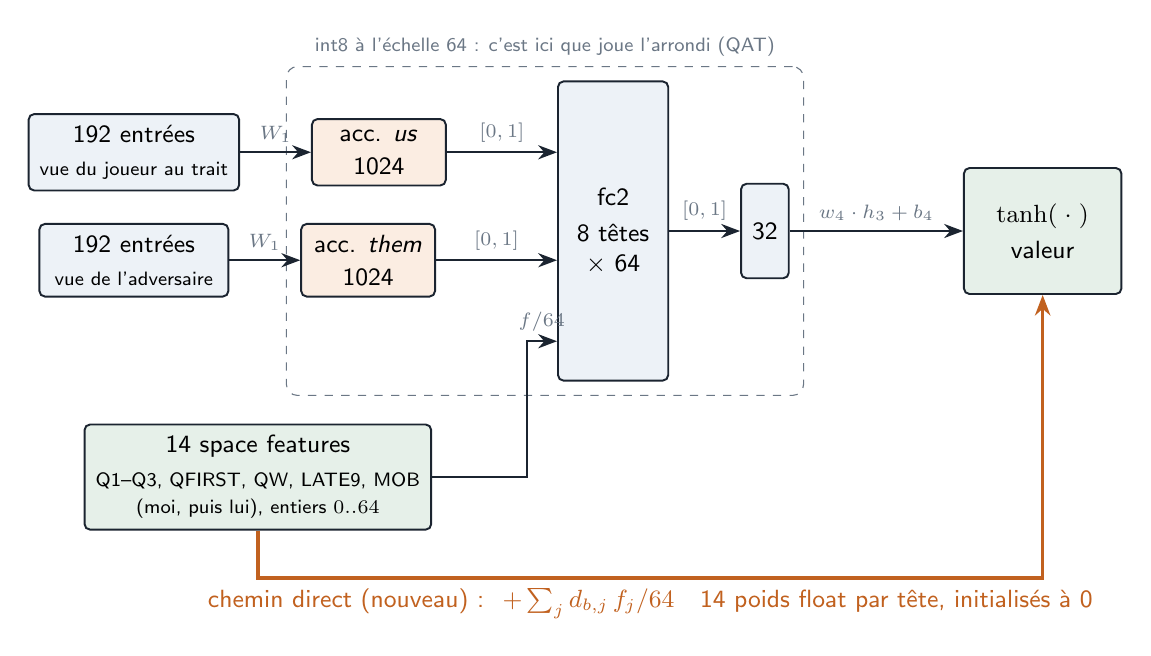
\begin{tikzpicture}[node distance=7mm]
  % the two points of view
  \node[box,minimum width=24mm] (us) {192 entrées\\[1pt]\scriptsize vue du joueur au trait};
  \node[box,minimum width=24mm,below=4mm of us] (them) {192 entrées\\[1pt]\scriptsize vue de l'adversaire};
  \node[boxa,right=9mm of us,minimum width=17mm] (accu) {acc. \textit{us}\\[1pt]1024};
  \node[boxa,right=9mm of them,minimum width=17mm] (acct) {acc. \textit{them}\\[1pt]1024};
  \draw[ar] (us) -- node[tiny,above]{$W_1$} (accu);
  \draw[ar] (them) -- node[tiny,above]{$W_1$} (acct);
  % space features
  \node[boxb,below=16mm of acct,minimum width=17mm,xshift=-14mm] (sp) {14 space features\\[1pt]\scriptsize Q1–Q3, QFIRST, QW, LATE9, MOB\\[-1pt]\scriptsize (moi, puis lui), entiers $0..64$};
  % fc2 per head
  \node[box,right=14mm of accu,yshift=-10mm,minimum height=38mm,minimum width=14mm] (h2) {fc2\\[2pt]8 têtes\\$\times$ 64};
  \draw[ar] (accu.east) -- node[tiny,above]{$[0,1]$} (h2.west |- accu.east);
  \draw[ar] (acct.east) -- node[tiny,above]{$[0,1]$} (h2.west |- acct.east);
  \draw[ar] (sp.east) -- ++(12mm,0) |- node[tiny,pos=0.75,above]{$f/64$} ([yshift=-14mm]h2.west);
  \node[box,right=9mm of h2,minimum height=12mm] (h3) {32};
  \node[boxb,right=22mm of h3,minimum height=16mm,minimum width=20mm] (v) {$\tanh(\;\cdot\;)$\\[2pt]valeur};
  \draw[ar] (h2) -- node[tiny,above]{$[0,1]$} (h3);
  \draw[ar] (h3) -- node[tiny,above]{$w_4\cdot h_3 + b_4$} (v);
  % the direct path
  \draw[-{Stealth[length=2.6mm]},draw=accent2,line width=1.3pt]
       (sp.south) -- ++(0,-6mm) -| node[pos=0.25,below,font=\sffamily\small,text=accent2]
       {chemin direct (nouveau) : \;$+\sum_j d_{b,j}\, f_j/64$\quad 14 poids float par tête, initialisés à 0}
       (v.south);
  % the int8 part
  \begin{scope}[on background layer]
    \node[fit=(accu)(acct)(h2)(h3),draw=muted,dashed,rounded corners=4pt,inner sep=5pt,
          label={[tiny]above:int8 à l'échelle 64 : c'est ici que joue l'arrondi (QAT)}] {};
  \end{scope}
\end{tikzpicture}
\end{document}
